%================================================================================
%       Safety Critical Systems Club - Data Safety Initiative Working Group
%================================================================================
%                       DDDD    SSSS  IIIII  W   W   GGGG
%                       D   D  S        I    W   W  G   
%                       D   D   SSS     I    W W W  G  GG
%                       D   D      S    I    WW WW  G   G
%                       DDDD   SSSS   IIIII  W   W   GGG
%================================================================================
%               Data Safety Guidance Document - LaTeX Source File
%================================================================================
%
% Description:
%   Appendix regarding Dazzle / distracting / disruptive data
%   Originally typeset from draft 0.5 and later updated to 0.7
%================================================================================
\section{Dazzle Data and Safety (Informative)}\index{Dazzle Data|textbf}\index{Data!Dazzle|see{Dazzle Data}} \label{bkm:dazzledata}
%
%\dsiwgSectionQuote{A ship in a port is safe, but that's not what ships are built for}{Grace Hopper}

%\dsiwgSectionQuote{Don't fix the blame, fix the problem}{Keith Pennington}

\dsiwgSectionQuote{Camouflage is a game we all like to play, but our secrets are as surely revealed by what we want to seem to be as by what we want to conceal}{Russell Lynes}

\subsection{Introduction}
This appendix outlines some of the safety implications arising from the issues identified by
``Dazzle Data'' in contrast to ``Dark Data''\index{Dark Data} presented in David Hand's book:
``Dark Data: Why What You Don't Know Matters'' \cite{citation:darkdata:hand}
and website \cite{citation:darkdata:website}.
Dark Data\index{Dark Data} relates to data that is not available but nevertheless is important.

``Dazzle Data'' refers to spurious, superfluous or unexpected data that masks and confuses the picture and can reduce your ability to see details, and indeed the whole picture --- a bit like noise or camouflage.

\begin{quote}
  It is data you don't want, didn't ask for, arrives more frequently than expected, is redundant, or data that arrives at an unexpected or inconvenient time or in the wrong format or sequence, so requiring extra resources to deal with\dots
\end{quote}

At first sight it might be thought this is just an annoyance rather than a problem,
however Dazzle Data can mask, distort or prevent usage of the real or desired data.
It can hide the true picture as in ``wood for the trees'' and in the worst case create real problems. 

Some examples of such false positive alerts that cause real alerts to be ignored are:
\begin{itemize}
  \item The classic case of ``Crying Wolf''.
  \item Denial of Service Attack, when servers can be blocked with useless requests that cannot be distinguished from the real requests.
\end{itemize}

Data which is truly spurious and believable (e.g. generated by extensive electrical noise, or fabricated to mask a fraud) may be accepted as valid data, leading to potentially hazardous results. 

Varieties of Dazzle Data may be identified\index{Dazzle Data} in the same grid manner as Dark Data\index{Dark Data}, as shown in \autoref{fig:dazzle}, where the yellow areas indicate potential dazzle data.

\begin{figure}[htbp]
  \centering
  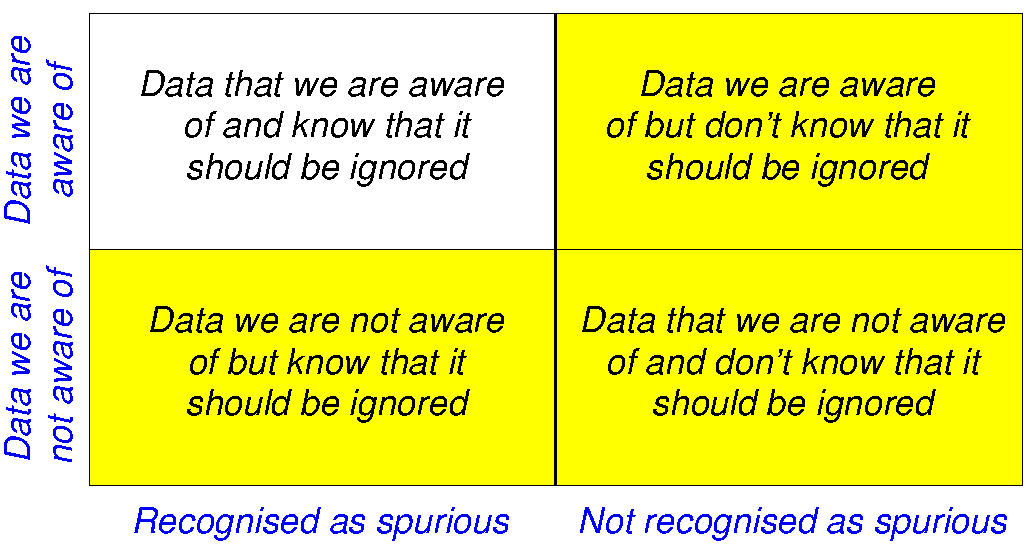
\includegraphics[width=\textwidth/2]{images/dazzleknowns.pdf}
  \caption{Dazzle data varieties}
  \label{fig:dazzle}
\end{figure}

\clearpage
\subsection{Dazzle Data Examples}

\subsubsection{Data We Are Aware Of --- Recognized as Spurious}\index{Dazzle Data!Data We Know are Spurious or Unneeded}
Repeated false positive alerts (e.g. from faulty sensors or alarms). These tend to be annoying irritants rather than safety issues, however they can lead to alarms being permanently switched off, masking true problems. An example from everyday life might be removing the battery from a badly place smoke alarm in a kitchen which repeatedly sounds when the toaster is used.

\subsubsection{Data We Are Aware Of --- Not Recognized as Spurious}\index{Dazzle Data!Data We Don't Know are Spurious or Unneeded}
Electromagnetic interference (EMI) affecting transmitted data is a good example of this case; we know it exists as a possibility but don't know how it might affect data in a system or a communications path, and this could be in different ways at different times or days.

\subsubsection{Data We Are Not Aware Of --- Recognized as Spurious}\index{Dazzle Data!Data We Know are Spurious or Unneeded}
In many cases we do not know what changes or corruptions may affect the data, but we have strong correction mechanisms to cope with the problems regardless. A good example is data stores on a spacecraft which have redundancy and error correcting codes built-in and so can deal with the majority of corruptions caused by cosmic rays.

\subsubsection{Data We Are Not Aware Of --- Not Recognized as Spurious}\index{Dazzle Data!Data We Don't Know are Spurious or Unneeded}
An example of this is where data is mistakenly added to a machine learning training data\index{Machine Learning Data} set resulting in bizarre and possibly hazardous behaviours of the system using it (e.g. an autonomous road vehicle). It is paramount that data used for such image recognition systems filters and excludes potentially dangerous extraneous data arising from unanticipated situations 

\subsection{Dazzle Data Varieties\index{Dazzle Data} and Safety Examples}
In his book, David Hand introduces a taxonomy of fifteen varieties of Dark Data\index{Dark Data}. This section discuses each form of Dazzle Data and considers it from a systems and safety assurance perspective.
Some of the varieties are the same as Dark Data\index{Dark Data}, but some are very different.

\subsubsection{Data We Know are Superfluous or Unneeded: ``Known Extras''}\index{Dazzle Data!Data We Know are Spurious or Unneeded|textbf}
\label{bkm:dazzledata:case1}

This case is very common in systems where an interface\index{Interface!Flooding} may be flooded with unsolicited messages.
It is also common in  safety justifications\index{Justification, Safety} where assurance information may be padded out with extra, irrelevant information that can mask the underlying safety argument (which may or may not be intentional).
It can be a serious problem in large, complex safety documents or detailed safety analyses.
Luckily, in this case, the data is recognized as superfluous and can be ignored.
Common examples include:
\begin{itemize}
    \item Mailboxes filled with spam mail, preventing important messages being read
    \item Repeated stall warnings when the aircraft is under control
    \item Assurance information in a safety case is included for components which are not part of the solution in use at that site or situation
    \item Assurance information about old or legacy components is included but these are now not in service
    \item Machine learning training data\index{Machine Learning Data} contains many cases which are duplicates or very closely related, so adding nothing to the learned behaviour but making the set hard to deal with
\end{itemize}
This case can be mitigated\index{Mitigation} in several ways, including careful filtering, review, use of concise  notations (such as Goal Structuring Notation) to extract the essence, and periodic audits and cleans. 

\subsubsection{Data We Don’t Know Are Unneeded or Spurious: ``Unknown Extras''}\index{Dazzle Data!Data We Don't Know are Spurious or Unneeded|textbf}
This is the most serious and far-reaching case, where the additional data is not recognized as unneeded and may be processed, analysed or be left in place when it should be removed. Some examples are:
\begin{itemize}
\item Legacy code in software\index{Software!Legacy} where nobody understands its function, or how it relates to the current code and so is reluctant to remove it. The Ariane 4 Inertial Reference function left in place in the Ariane 501 launch disaster might be such a case. Note that code whose function is known would be under the first case, discussed in \ref{bkm:dazzledata:case1}
    \item Parts of the safety case or safety argument are supplied separately (e.g. by a subcontractor or 3rd party) and they are obscure. In this case it will not be known which parts are relevant to the particular situation. Some information may be irrelevant or worse, misleading.
    \item Machine learning training data\index{Machine Learning Data} containing too many outliers, which are not recognized as such
\end{itemize}

In many cases the extra data may be discovered after some time, and it is incumbent on the organization involved to analyse the impact of the complete set of data which may have been used over the time period, including subsequent decisions and actions. The effect of spurious data should not be underestimated, as it may have masked, prevented or distorted the intended use of the nominal data for some time. This case can fundamentally change the safety picture and is probably in the highest safety risk category.

Data found to be erroneous (i.e. it should not ever have been in the system or in the safety argument) is a problem. The following options show possible approaches to handling this data:
\begin{enumerate}[label=\color{dsiwgAccentColour}\roman*)]
    \item Delete the erroneous data
    \item Accept the erroneous data, i.e. continue using it
    \item Report that the data was erroneous but take no further action 
    \item Establish under what circumstances and situations the erroneous data would have had an effect
    \item Perform a full impact analysis on the effects of the erroneous data and then act according to the results
\end{enumerate}

\subsubsection{Data Obscuration: Missing What Matters}\index{Dazzle Data!Data Obscuration}
This is where the meaning of the overall data set becomes obscured due to the extra unnecessary data. Examples might be:
\begin{itemize}
    \item Measuring the wrong things due to excessive noise or too much data to deal with
    \item Processing involving sampling only picks bad data elements
    \item Being too close to the data, i.e. the ``wood for the trees''. This is when the extra data masks the overall issue with the data, e.g. a slow trend or bias hidden by large local variations.
\end{itemize}

Mitigations\index{Mitigation} include review, statistical checks and ``taking a step back'' to look at the bigger picture.
\subsubsection{Data Masking in Specific Cases}\index{Dazzle Data!Data Masking in Specific Cases}
This is where the extra data specifically masks, obscures or hides particular data elements (but not all). A particularly nasty case of this is where filters are put in place to remove unwanted data values, but those filters actually remove less (or more) than they should (i.e. don’t remove all unwanted cases or remove valid values as well). Some examples might be:
\begin{itemize}
    \item The number of successful test runs vastly outweighs failed runs and so the failures are not investigated
    \item Incorrect filtering of the data, leaving in some cases that should have been excluded
\end{itemize}

Mitigations\index{Mitigation} include use of review and \index{Completeness!Checks}completeness checks. Note that over-aggressive filtering would create cases of Dark Data\index{Dark Data}.
\subsubsection{Masquerade or Fraudulent Data}\index{Dazzle Data!Masquerade or Fraudulent Data}
This is where data has been constructed to fool the system consuming it, hiding, overlaying or replacing the correct data. Often this will be malicious and should be filtered or rejected by the target system, but of course may not be. 
\begin{itemize}
    \item Intentional fraud
    \item Some security attacks
\end{itemize}

Mitigations\index{Mitigation} include audit, blockchain, monitoring, intelligent profiling of data and detection of changes.

\subsubsection{Incorrect Definitions of Data}\index{Dazzle Data!Incorrect Definitions of Data}
This is considered a common case for systems exchanging data with external systems, where they may duplicate, translate or incorrectly send multiple messages. They may be time-separated, for instance if communications are lost and then regained, leading to confusion.
\begin{itemize}
    \item Data sent in the wrong rate or units (e.g. every millisecond rather than second)
    \item Data given for the wrong range or duration (e.g. for a month rather than a day
    \item Data sent for the wrong domain or scale (e.g. national values rather than regional)
    \item Text messages re-sent to a mobile phone when coverage restored
\end{itemize}

Mitigations\index{Mitigation} include making sure interface\index{Interface!Specification} specifications are clear and ambiguous, rejecting incorrect size or scale data sets, keeping a list of known changes / incompatibilities and documenting the changes or fixes that have to be applied to make the data usable or consistent.

\subsubsection{Summaries of Data}\index{Dazzle Data!Summaries of Data}
Spurious data can affect summaries in a significant way if composite values are calculated, e.g.
\begin{itemize}
    \item Calculations of averages or other statistics affected by duplicates
    \item Spurious outliers can lead to overfitting when analysing data trends
\end{itemize}

Mitigations\index{Mitigation} include audit and assessing what extra data could cause (i.e. performing sensitivity analysis) and establishing what decisions might be made erroneously due to certain data values being present.	

\subsubsection{Information Asymmetry}\index{Dazzle Data!Information Asymmetry}
This is common where there are multiple stores or sources of the same data. If one has erroneous duplicate values (i.e. many null values used for padding) then comparisons between them may fail.
\begin{itemize}
    \item Multiple / backup databases where they are not kept in sync
    \item Issues of divergence of data across multiple sources.
\end{itemize}

Comparisons, reviews and data audits may help in these cases. In general the issue of divergence across multiple data sources needs to be recognized and addressed in an automated way.

\subsubsection{Intentionally Dazzled Data}\index{Dazzle Data!Intentionally Dazzled Data}
This might happen in a secure context where key data is effectively ``camouflaged'' by hiding within large data items (e.g. images) or the use of large amounts of apparently routine data to mask the secure data.
\begin{itemize}
    \item Defence, security and government sectors where data is purposefully hidden 
    \item An organization may provide copious amounts of safety case collateral to hide a weak safety case
\end{itemize}
\subsubsection{Extrapolating Beyond Your Data}\index{Dazzle Data!Extrapolating Beyond your Data}
Machine learning systems have to cope with values outside of their training data\index{Machine Learning Data}, but the outcomes may be unexpected if the training data contains many spurious values:
\begin{itemize}
    \item Bizarre results from recognition / detection systems due to out of range values
    \item Image components mislabelled leading to strange results
\end{itemize}

Mitigations\index{Mitigation} include checking of the values that are used in training, analysis of outliers and repeats, deletion of duplicates and use of machine learning validation data\index{Machine Learning Data} containing edge/corner cases and boundary cases.

\paragraph{A Note on Sensors}
Sensors can degrade and fail over time, especially in harsh environments such as automotive, marine or aviation. In such cases sensors may feed erroneous or additional data into systems (e.g. if an out of normal range situation is detected), leading to misleading processing or false alarms. The \index{Boeing 737}Boeing 737 MAX~8 accidents might fall into this category as the angle-of-attack sensor erroneously generated high values, and certainly the systems/processing which passed on the values created spurious data. Some examples are:
\begin{itemize}
    \item Faulty sensors
    \item Multiple sensors that do not have their values properly combined
    \item Sampling techniques which generate additional data
    \item Interval polling interval can lead to misleading readings
    \item Data fusion can be impacted if multiple sensor values are combined
\end{itemize}

Mitigations\index{Mitigation} include independent monitoring of sensors and regular maintenance, calibration or replacement of hardware. Their interfaces\index{Interface!Sensor} need to be able to detect any problems and report faults. In particularly critical applications, it may be necessary to minimise the potential for common mode failures by using disparate technologies, or at least sensors from different manufacturers.

An example may be found in\index{Qantas}
\href{https://en.wikipedia.org/wiki/Qantas\_Flight\_72}{https://en.wikipedia.org/wiki/Qantas\_Flight\_72}
where:
\begin{quotation}
  \dots the \acrshort{cpu}\footnote{\acrlong{cpu}} of the \acrshort{adiru}\index{ADIRU}\footnote{\acrlong{adiru}} corrupted the \acrfull{aoa} data. The exact nature of the corruption was that the \acrshort{adiru} \acrshort{cpu} erroneously re-labelled the altitude data word so that the binary data that represented 37,012 (the altitude at the time of the incident) would represent an angle of attack of 50.625 degrees. The \acrshort{fcpc}\footnote{\acrlong{fcpc}} then processed the erroneously high \gls{aoa} data, triggering the high-\gls{aoa} protection mode, which sent a command to the electrical flight control system (EFCS) to pitch the nose down.
  
  The \acrshort{fcpc} algorithm was very effective, but it could not correctly manage a scenario where there were multiple spikes in either \gls{aoa} 1 or \gls{aoa} 2 that were 1.2 seconds apart --- i.e., if the 1.2-second period of use of the memorised value happened to end while another spike was happening.
  \end{quotation}

\subsection{Summary}
Dazzle Data is a very useful way of thinking about data problems and solutions.
It is important to always think of the bigger picture,
considering what information is superfluous and may be distorting or masking the real picture:
\begin{itemize}
    \item What might be hidden intentionally or otherwise due to the extra values?
    \item Could the extra items cause any safety problems, e.g. change a numerical calculation?
    \item How would a system cope if it received data it was not expecting?
    \item How do you characterise the nature of unexpected data so as to ensure it can be handled if it does occur?
    \item Can you present your results / outputs in a way that shows the extra data?
\end{itemize}

Fundamentally, Dark Data is data that is not available, but nevertheless is important, and indeed, in some cases, more important than the data that is available.

Similarly, Dazzle Data refers to spurious, superfluous or unexpected data that masks and confuses the picture and
can reduce your ability to see details, and indeed the whole picture --- a bit like noise or camouflage.

The opposite attributes of dark data and dazzle data might be termed Brightness and Clarity respectively. These are potential new properties or meta-properties of data.

\begin{longtable}{|L{\dsiwgColumnWidth{0.17}}|L{\dsiwgColumnWidth{0.17}}|C{\dsiwgColumnWidth{0.17}}|C{\dsiwgColumnWidth{0.17}}|L{\dsiwgColumnWidth{0.32}}|}
  \caption{A comparison of Dark and Dazzle data properties}
  \label{tab:DarkDazzleComparison}
  \\\hline\TableHeadColour{Data Property} & \TableHeadColour{Explanation} & \TableHeadColour{Dark Data --- missing data} & \TableHeadColour{Dazzle data --- obscuring data} & \TableHeadColour{Notes}\\\hline
  \endfirsthead
  \caption[]{A comparison of Dark and Dazzle data properties (continued)}
  \\\hline\TableHeadColour{Data Property} & \TableHeadColour{Explanation} & \TableHeadColour{Dark Data --- missing data} & \TableHeadColour{Dazzle data --- obscuring data} & \TableHeadColour{Notes}\\\hline
  \endhead
  \multicolumn{5}{r}{\sl Continued on next page}
  \endfoot\endlastfoot
  %
  Integrity (I) & The data is correct, true and unaltered & \tick & \tick &
  E.g., Corruptions to a database could change the original values so the original data is lost, or hide or mask values such as by inserting End-of-File markers\\
  \hline
  %
  Completeness (C) & The data has nothing missing or lost & \tick & - &
  If data is lost then it is usually unknown and hence dark. However use of parity, CRCs and digital signatures may be able to detect the loss and, in some cases, fill in the missing data.\\
  \hline
  %
  Consistency (N) & The data adheres to a common world view (e.g., units) & - & - &\\
  \hline
  %
  Continuity (Y) & The data is continuous and regular without gaps or breaks & \tick & - &
  Gaps or breaks in a data stream would be dark --- the missing values are unknown.
  Methods may be available to mitigate if detected, e.g., interpolation.\\
  \hline
  %
  Format (O) & The data is represented in a way which is readable by those that need to use it & \tick & \tick &
  If data is not in the correct format then it may not be usable so becomes dark. If lots of data is in the wrong format it may obscure other (good) data, and hence can dazzle.\\
  \hline
  %
  Accuracy (A) & The data has sufficient detail for its intended use & \tick & - &
  If the data has lost detail (e.g., due to sensor sampling or representation) then this is a dark case.\\
  \hline
  %
  Resolution (R) & The smallest difference between two adjacent values that can be represented
  in a data storage, display or transfer system & \tick & \tick &
  If the system cannot distinguish between different data values that actually are different, then data could become hidden or lost and hence dark. If the data is masked then it may also be a case of dazzle data.\\
  \hline
  %
  Traceability (T) & The data can be linked back to its source or derivation & \tick & - &
  If traceability is lost then the data effectively becomes darker as its origins and derivation are lost, and may not be able to be used.\\
  \hline
  %
  Timeliness (M) & The data is as up to date as required & \tick & \tick &
  If data is not, or thought to be not, up to date then it may be rejected and hence become dark data. But clocks can become out of sync across different systems leading to erroneous rejection so the timestamps may then be thought of as dazzling the system.\\
  \hline
  %
  Verifiability (V) & The data can be checked and its properties demonstrated to be correct & \tick & - &
  If data can’t be checked then it may be rejected (and become dark), even if it is valid.\\
  \hline
  %
  Availability (L) & The data is accessible and usable when an authorized entity demands access & \tick & - &
  If data is not available as required then it is dark (whether it exists or not).\\
  \hline
  %
  Fidelity / Representation (F) & How well the data maps to the real-world entity it is trying to model &
  - & - &\\
  \hline
  %
  Priority (P) & The data is presented / transmitted / made available in the order required &
  \tick & \tick &
  If data is not prioritised to be available when needed it is effectively dark. This could be because other data is taking precedence so could be a dazzle case.\\
  \hline
  %
  Sequencing (Q) & The data is preserved in the order required &
  \tick & \tick &
  If data is not sequenced as needed it may be rejected or ignored and then is effectively dark. Other data which is out of order or sequence may cause the whole message, set or file to be rejected – a dazzle case.\\
  \hline
  %
  Intended Destination / Usage (U) & The data is only sent to those that should have access to it &
  \tick & - &
  If data is not sent to the correct destination it may be a dark data situation as it is effectively missing.\\
  \hline
  %
  Accessibility (B) & The data is visible only to those that should see it &
  - & \tick &
  If data is more widely visible or distributed than intended it could cause a dazzle situation due to e.g. bandwidth issues.\\
  \hline
  %
  Suppression (S) & The data is intended never to be used again &
  - & \tick &
  If data re-emerges after it should have been deleted it could cause all sorts of dazzle-related problems.\\
  \hline
  %
  History (H) & The data has an audit trail of changes &
  \tick & - &
  If the audit trail is lost then the data is darkened as its origins and derivation could be important.\\
  \hline
  %
  Lifetime (E) & When does the safety-related data expire &
  \tick & \tick &
  If the lifetime is erroneously early than the data is lost --- a dark data problem. Conversely if the lifetime is too long it is potentially a dazzle situation.\\
  \hline
  %
  Disposability / Deletability (D) & The data can be permanently removed when required &
  - & \tick &
  If the data cannot be removed it is potentially a dazzle situation, as it may obscure the real or current data.\\
  \hline
  %
  Goldilocks (G) & The data is just the right size — not too much and not too little &
  \tick & \tick &
  Too little data may be a dark data case and too much data to deal with is a dazzle case.\\
  \hline
  %
  Analysability (Z) & The data is of a suitable size, type and representation (including any metadata) to enable it be usefully analysed &
  \tick & \tick &
  If the data can’t be analysed it may not be able to be used causing a dark data issue. If there is too much of it or it is obscured (e.g., by noise on a comms line) then it is a dazzle case.\\
  \hline
  %
  Explainability (X) & The data can be meaningfully explained to those who need to understand it by a suitable mechanism &
  \tick & \tick &
  If the data can’t be explained it may not be able to be used causing a dark data issue. If there is too much of it or suitable management and analysis tools are not available then it is potentially both cases.\\
  \hline
  %
\end{longtable}
